

\subsection{API and guarantees}

\sys\ is a persistent key-value store supporting \emph{put, get}, and atomic \emph{range scan} (or scan) operations. 
Scans are atomic in the sense that all values returned by a single scan belong to a consistent snapshot reflecting
the state of the data store at a unique point in time.

\Idit{More on API?}

\sys\ ensures \emph{durability} of all updates by writing updates to disk synchronously as part of the \emph{put} operation.

\subsection{Data organization}

\begin{figure}[htb]
\centerline{
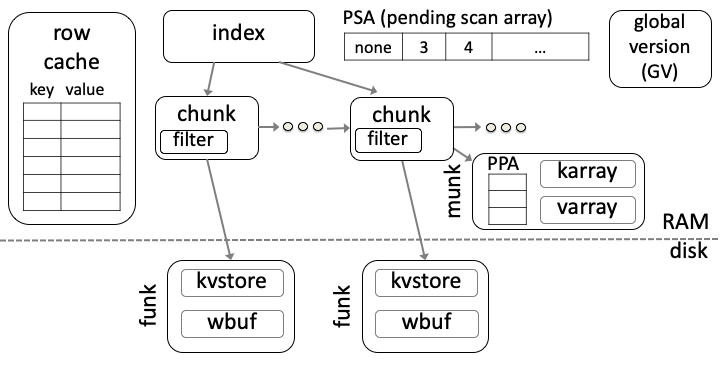
\includegraphics[width=0.9\columnwidth]{PiWi.png}
}
\caption{\sys\ data layout.}
\label{fig:layout}
\end{figure}

\paragraph{Chunk-based layout.}

\sys's data layout is depicted in Figure~\ref{fig:layout}.
Similarly to BTrees \Idit{and other disk-friendly data structures?}, 
\sys\ organizes data in fixed-size \emph{chunks}, each holding a contiguous key range.
At run-time, a list of all chunks is kept in RAM, where each chunk's data 
(consisting of keys in the corresponding range and values associated with them) 
is kept on disk (for persistance), and possibly in memory (for fast access). 

More specifically, each chunk is associated with a \emph{file chunk}, or \emph{funk},
which is a persistent data structure consisting of three files holding the chunk's data -- a value store \emph{vstore}, 
a sorted key store \emph{kstore}, and a write buffer \emph{wbuf}. The vstore holds all the values associated with keys
in the chunk. When a funk is created, the kstore holds all the chunk's keys with pointers to corresponding values.
New keys are subsequently appended to the unsorted wbuf, while new values are appended to the chunk's vstore.
This strucutre allows us to update chunks without re-writing existing data, thus minimizing write amplification.

Since updates to disk are executed synchronously,  the data store reflecting all completed put operations 
can be consistently recovered from the on-disk funks at any time. \Idit{Need to discuss recovery somewhere.}

A subset of the chunks is also cached in memory to allow fast access, each in a data structure called \emph{memory chunk (munk)}. 
A munk consists of two arrays, kstore and vstore, where the kstore is organized as a sorted linked list. 
Updates are performed in place. Munks are volatile and can be removed and recreated from funks at any time.
Thus, multiple \emph{generations} of munks may exist for a chunk throughout its life time.

At run-time, \sys\ holds in memory a linked list of chunk objects representing all funks in the data store. 
Chunks are also indexed in-memory for fast access by key using an in-memory sorted map (e.g., a skip list or search tree).
Note that since chunk objects do not hold actual keys and values, they are significantly smaller than munks and funks. 
\inred{A typical chunk object is smaller than 1KB, whereas the size of a funk or munk that holds 10K to 100K keys 
ranges between 1M to 100M depending on the data size. A typical \sys\ node holds thousands of chunks, with 
all chunk obejcts in memory in addition to hundreds of munks.} 

As key-value pairs are added, overwritten, and removed, chunks need to undergo reorganization. This includes  
\emph{compaction} to deallocate removed and overwritten data, 
\emph{sorting} keys to make searches more efficient,  
\emph{splitting} overflowing chunks, and
\emph{merging} under-utilized ones.
All reorganizations are performed by \sys's \emph{reblance} operation.
Rebalance compacts and sorts a munk in-memory, by creating a new (compacted and sorted) munk instead of the existing one. 
Funks are also compacted by replacing them with new funks, albeit less frequently.
Splits and merges create new chunks as well as the munks and funks associated with them.

\paragraph{Multi-versioning.}

We support atomic scans via multi-versioning using a system-wide \emph{global version (GV)}. 
A scan operation creates a \emph{snapshot} associated with GV's current value by incrementing GV, 
which signals to ensuing put operations that they must not overwrite values associated with 
smaller versions than the new GV value.
This resembles a \emph{copy-on-write (CoW)} approach, which virtually creates a snapshot by 
indicating that data pertaining to the snapshot should not be modified in place.  
To allow garbage collection of old versions that are no longer required for any active scan, \sys\ also maintains 
a \emph{pending scan array (PSA)}, with one entry per active thread, tracking snapshot times of ongoing scans.

For linearizing updates, we associate each key-value pair written to the data store with a unique-per-key identifier.
This identifier is a truple $\langle$ver, gen, i$\rangle$, where \emph{ver} is  the version read from GV 
(recall that GV is only incremented upon scans and hence might remain unchanged across multiple puts),
\emph{gen} is the generation of the last munk created in the corresponding chunk
(which may or may not still exist), 
and \emph{i} is a running sequence number of values inserted to the chunk in the current generation.
In case the munk exists, $i$ is the 
index of the cell holding the key in the munk's kstore as well as the cell holding the value in the munk's vstore. 

\paragraph{Data structure.}

The chunk data structure is given in Algorithm~\ref{alg:chunk}. 
It holds a pointer to the appropriate funk, and, if applicable, also munk. 
It further keeps the generation number of its latest munk and the index,
which, in case there is an active munk, is the index of the next free cell in the munk's kstore and vstore.

The chunk additionally includes locks and data structures to synchronize concurrent access by multiple threads.
The replacement of a chunk (due to a split or a merge) or of a funk or munk associated with a given chunk 
must be executed atomically, and moreover, must be synchronized with concurrent puts. 
This is controlled by the chunk's rebalance\_lock, which is held for short time periods
during chunk/funk/munk replacements.  It is a read/write (shared/exclusive) lock, acquired in shared mode 
by put opertaions and in exclusive mode by rebalance. \Idit{What about gets?}

To minimize I/O, we allow at most one thread to rebalance a funk at a given time; this is controlled by 
the  funk\_change\_lock. This lock is used at a coarse granularity -- it is held throughout the creation of the new funk. 
Finally, the chunk holds a data structure called PPA for synchronizing concurrent puts, as will be explained below. 


\begin{algorithm}[htb]
\begin{algorithmic}
\State ptr funk \Comment funk disk address
\State ptr munk \Comment munk memory pointer
\State int gen \Comment munk generation
\State int i \Comment munk index
\State r/w lock rebalance\_lock \Comment asymmetric  lock 
\State lock funk\_change\_lock \Comment conventional lock 
\State PPA[threads] \Comment pending put array
\end{algorithmic}
\caption{Chunk data structure.}
\label{alg:chunk}
\end{algorithm}







%Since \sys\ is geared towards analytics workloads, which emphasize long range scans, we organize it as a sorted data structure.

